\documentclass{ctexart}

\usepackage{palatino}
\usepackage{tikz}
\usetikzlibrary{shapes.geometric, arrows}
\usepackage{bm}
\usepackage{geometry}
\usepackage{titlesec} %自u格式的宏包
\usepackage{picinpar,graphicx}
\usepackage{zhnumber}
\usepackage{float}
\usepackage{caption,subcaption}
\usepackage{amsmath}
\usepackage{amssymb}
\usepackage{fancyhdr}%页眉页脚
\usepackage{multirow}
\usepackage{upgreek}
\usepackage{paralist}
\usepackage{diagbox,array}
\usepackage{cite}
\usepackage{minted}
\usepackage{listings}
\usepackage{xcolor}
\usepackage{hyperref}
\usepackage{tabularx}
\usepackage{booktabs}
\usepackage{fancyhdr}
\usepackage{verbatim}

\lstset{
	basicstyle=\small,%
	escapeinside=``,%
	keywordstyle=\color{red} \bfseries,% \underbar,%
	identifierstyle={},%
	commentstyle=\color{blue},%
	stringstyle=\ttfamily,%
	%labelstyle=\tiny,%
	extendedchars=false,%
	linewidth=\textwidth,%
	numbers=left,%
	numberstyle=\tiny \color{blue},%
	frame=trbl%
}

\geometry{a4paper,left=0.75in,right=0.75in,top=1in,bottom=1in} %页边距


%\counterwithin{figure}{section}
%\counterwithin{table}{section}
\counterwithin{equation}{section}

\renewcommand{\thefigure}{ \arabic{figure}}
\renewcommand{\thetable}{\arabic{table}}
\renewcommand{\theequation}{ \arabic{section}-\arabic{equation}}
\renewcommand \thesection {\arabic{section}}
\renewcommand \thesubsection {\arabic{section}.\arabic{subsection}}
\renewcommand{\caption}[1]{\caption[\songti\ziju{-5}]{#1}}
%\\totalnumber{10}
%\renewcommand{\thesubfigure}{\arabic{section}-\arabic{figure}-\arabic{subfigure}}

\titleformat{\section}[block]{\zihao{3}\bfseries}{\zhnum{section}、}{0em}{}[]
\titleformat{\subsection}[block]{\zihao{4}\bfseries}{\quad\arabic{section}.\arabic{subsection}}{0em}{}[]
\titleformat{\subsubsection}[block]{\zihao{-4}\bfseries}{\quad\quad\arabic{section}.\arabic{subsection}.\arabic{subsubsection}.}{0em}{}[]
%%\titleformat{\paragraph}[block]{\songti\zihao{5}}{[\arabic{paragraph}]}{1em}{}[]

\setlength{\baselineskip}{22pt}



\zihao{-4}
%\setlength{\parskip}{0.1pt}
\bibliographystyle{IEEEtran}

\pagestyle{fancy}%清除原页眉页脚样式
\fancyhf{} 
\fancyhead[C]{燕\space 山\space 大\space 学\space 三级项目设计说明书}

\rfoot[C]{\centering\thepage}

\begin{document}
	
	\begin{table*}[H]
		\centering
		\begin{tabular}{c|c|c|c|c}
			\hline
			小组成员 & 负责工作  & 成员贡献度自评得分&小组得分 & 备注\\
			\hline
			王嘉琪 & 资料查询、Mworks仿真、报告 & 80\% & \multirow{5}{*}{m}&倒立摆X方向受力为0\\
			\hline
			刘云峰 & 报告 & 5\% & &\\
			\hline
			张智萱 & 报告 & 5\% & &\\
			\hline
			庆学璞 & 报告 & 5\% & &\\
			\hline
			曾杰 & 报告 & 5\% & &\\
			\hline
		\end{tabular}
	\end{table*}
	\newpage
	\tableofcontents
	\newpage
	\section{前言}
		倒立摆是典型的多变量、高阶次 ，非线性、强耦合、自然不稳定系统。倒立摆系统的稳定控制是控制理论中的典型问题 ，在倒立摆的控制过程中能有效反映控制理论中的许多关键问题。
	\section{系统分析与模型建立}
		\subsection{系统分析}
			\subsubsection{一维倒立摆系统的物理模型}
				对倒立摆被控对象进行分析，其受力图如图\ref{fig:倒立摆系统隔离受力图}。
				\begin{figure}[H]
					\centering
					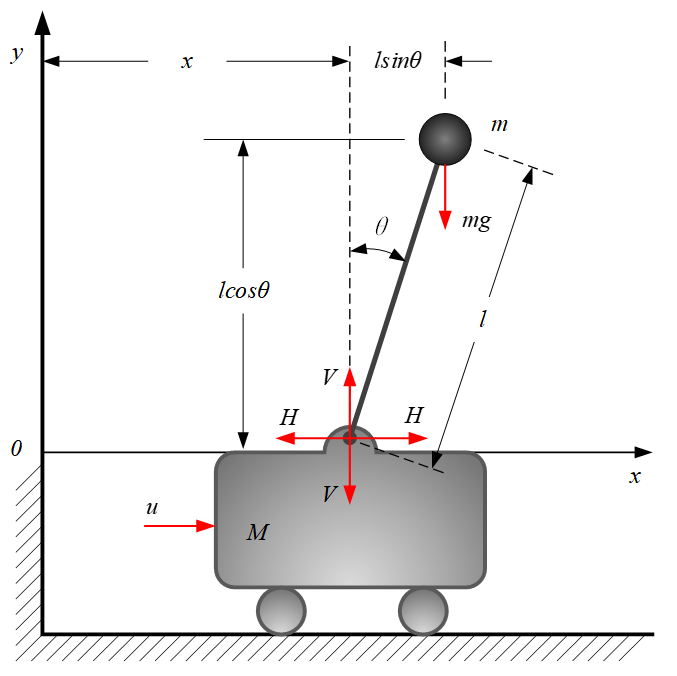
\includegraphics[width=0.4\linewidth]{倒立摆系统隔离受力图}
					\caption{倒立摆系统隔离受力图}
					\label{fig:倒立摆系统隔离受力图}
				\end{figure}
				可由图\ref{fig:倒立摆系统隔离受力图}看出，系统由小车，一根摆杆以及摆球组成，小车与摆杆之间由转轴相连。系统相关物理量如下表\ref{fig:符号变量表}：
				\begin{table}[H]
					\caption{符号变量表}
					\centering
					\begin{tabular}{c|c}
						\toprule%第一道横线
						符号 & 变量含义 \\
						\midrule%第二道横线 
						$M$ & 小车质量\\
						$m$ & 摆球质量\\
						$I$ & 摆杆绕其中心的转动惯量\\
						$L$ & 摆杆长度\\
						$g$ & 重力加速度\\
						$\theta$ & 倒立摆与竖直方向的夹角\\
						$u$ & 输入电压\\
						\bottomrule%第三道横线
					\end{tabular}
					\label{fig:符号变量表}
				\end{table}\par
				通过MWORKS的sysplorer搭建的一级倒立摆模型的物理模型。
				\begin{figure}[H]
					\centering
					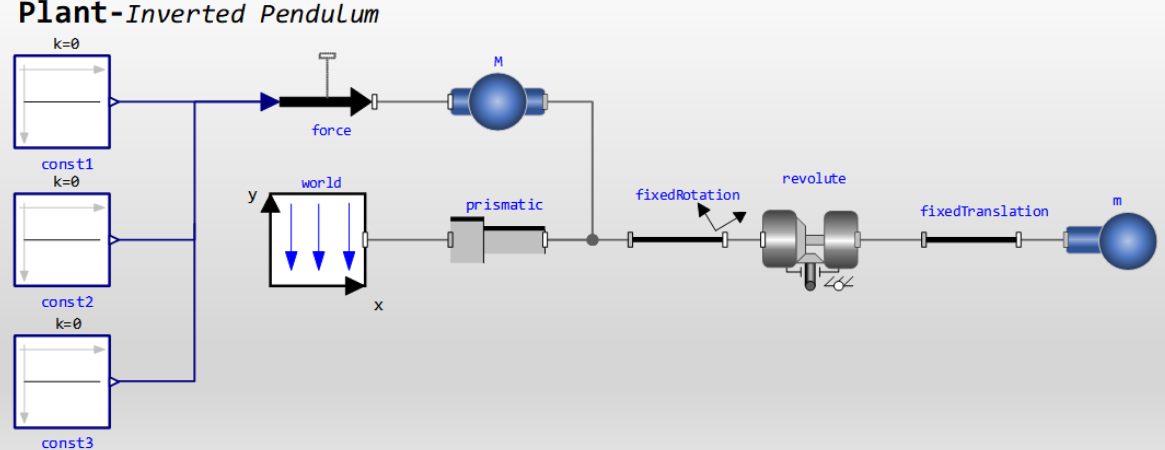
\includegraphics[width=0.9\linewidth]{倒立摆物理系统模型}
					\caption{倒立摆物理系统模型}
					\label{fig:倒立摆物理系统模型}
				\end{figure}
				\begin{table}[H]
					\caption{相关参数}
					\centering
					\begin{tabular}{c|c|c|c|c}
						\toprule%第一道横线
						符号 & 变量参数  & 值&单位 & 说明\\
						\midrule%第二道横线 
						const1 & $M$ & 0 & /&倒立摆X方向受力为0\\
						const2 & $M$ & 0 & /&倒立摆Y方向受力为0\\
						const3 & $M$ & 0 & /&倒立摆Z方向受力为0\\
						M & $m$ & 2 & kg&滑块质量为2kg\\
						\multirow{2}{*}{revolute} & $useAxisFlange$ &  & /&打开转动副外置法兰接口\\
						& $phi.tart$ &  10 & deg&摆动初始转角位$10^\circ$\\
						\multirow{2}{*}{m} & $r\_CM$ & $[0,0,5,0]$ & m&摆杆重心相对于转动副位置为$[0,0,5,0]$m\\
						 & $m$ & $0.1$ & kg&摆杆质量为$0.1$kg\\
						\bottomrule%第三道横线
					\end{tabular}
					\label{fig:相关参数}
				\end{table}
			\subsubsection{系统运动学模型的建立：空间表达式的建立}
				考虑摆杆重心的水平运动描述为：
				\begin{gather}
					m\frac{d^2}{dt^2}(x+l\sin \theta)=H
				\end{gather}\par
				摆杆重心的垂直运动描述为：
				\begin{gather}
					m\frac{d^2}{dt^2}(l\cos \theta)=V-mg
				\end{gather}\par
				小车的水平运动描述为：
				\begin{gather}
					M\frac{d^2x}{dt^2}=u-H
				\end{gather}\par
				再考虑摆杆转动，其绕重心（摆球重心）的转动运动可以描述为（$I$为摆杆绕其中心的转动惯量）：
				\begin{gather}
					I\frac{d^2\theta}{dt^2}=Vl\sin \theta-Hl\cos \theta
				\end{gather}\par
				根据上述非线性方程组可以描述一维倒立摆行为。当系统运作时保持倒立摆垂直可以理解为$\theta$角很小，因此可以近似为$\sin \theta \approx \theta$、$\cos \theta\approx 1$，再考虑到倒立摆围绕重心的转动惯量很小可以近似认为：$I\approx0$。\par
				考虑上述近似条件，非线性方程组可以被线性化，得到:
				\begin{gather}
					\begin{cases}
						(M+m)\ddot{x}+ml\ddot{\theta}=u\\
						ml^2\ddot{\theta}+ml\ddot{x}=mgl\theta
					\end{cases}
				\end{gather}\par
				将上式写成状态空间方程，定义以下状态变量：
				\begin{gather}
					\begin{cases}
						x_1=\theta\\
						x_2=\ddot{\theta}\\
						x_3=x\\
						x_4=\ddot{x}\\
					\end{cases}
				\end{gather}\par
				联立上面两组式子得到：
				\begin{gather}
					\begin{cases}
						\dot{x_1}=x_2\\
						\dot{x_2}=\frac{M+m}{Ml}gx_1-\frac{1}{Ml}u\\
						\dot{x_3}=x_4\\
						\dot{x_4}=-\frac{m}{M}gx_1-\frac{1}{M}u\\
					\end{cases}
				\end{gather}\par
				上式写成矩阵形式：
				\begin{gather}
					\begin{bmatrix}
						\dot{x_1}\\
						\dot{x_2}\\
						\dot{x_3}\\
						\dot{x_4}\\
					\end{bmatrix}
					=
					\begin{bmatrix}
						0&1&0&0\\
						\frac{M+m}{Ml}g&0&0&0\\
						0&0&0&1\\
						-\frac{m}{M}g&0&0&0\\
					\end{bmatrix}
					\cdot
					\begin{bmatrix}
						x_1\\
						x_2\\
						x_3\\
						x_4\\
					\end{bmatrix}
					+
					\begin{bmatrix}
						0\\
						-\frac{1}{Ml}\\
						0\\
						\frac{1}{M}\\
					\end{bmatrix}
					\cdot
					u\\
					y=
					\begin{bmatrix}
						0&0&1&0\\
					\end{bmatrix}
					\cdot
					\begin{bmatrix}
						x_1\\
						x_2\\
						x_3\\
						x_4\\
					\end{bmatrix}
				\end{gather}\par
				则得到了一维倒立摆系统的状态空间方程表达。
			\subsubsection{系统稳定性和能控能观性分析}
			稳定性分析：\par
			由系统的数学模型可以利用Mworks.Sysab平台的pzmap（）函数来绘制系统的零极点图，并以此来判断系统的稳定性。绘制结果如下图所示：
			\begin{figure}[H]
				\centering
				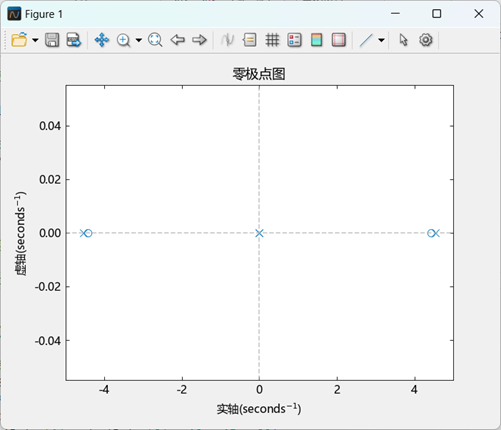
\includegraphics[width=0.6\linewidth]{系统的零极点图}
				\caption{系统的零极点图}
				\label{fig:系统的零极点图}
			\end{figure}\par
			由结果可知该系统在存在具有正实部的零极点，显然该系统是不稳定的。\par
			能控能观性分析：\par
			对于线性连续定常单输入系统，可通过能控性判别矩阵是否满秩来判断系统能观性：\par
			\begin{gather}
				M=
				\begin{bmatrix}
					B & AB& A^2B & \cdots &A^{n-1}B
				\end{bmatrix}
			\end{gather}\par
			同理，也可以通过能观性判别矩阵是否满秩来判断系统能观性：
			\begin{gather}
				M=
				\begin{bmatrix}
					C \\
					CA\\
					CA^2\\
					\vdots\\
					CA^{n-1}
				\end{bmatrix}
			\end{gather}\par
			首先Mworks.Sysab平台构建出能控能观判别矩阵。\par
			Co = ctrb(G)\par
			Ob = obsv(G)\par
			r1=rank(Co)\par
			r2=rank(Ob)\par
			再利用 Mworks软件的 rank 函数可以求得两个代入数据矩阵的秩，得到两矩阵均为满秩， 因此该系统为能控且能观的。
			
		\subsection{倒立摆控制律设计}
			控制律的设计目的是让倒立摆系统能够快速的在指定的位置（$x$）平衡（$\theta \rightarrowtail 0$），定义系统参数为：$M=2$kg、$m=0.1$kg、$l =0.5$m、$g=9.8$m/s$^2$，利用状态空间理论中的极点配置法进行控制律设计。
			\begin{figure}[H]
				\centering
				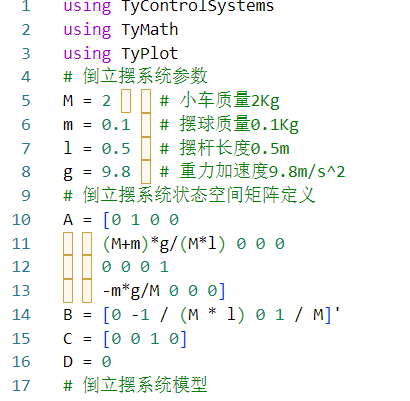
\includegraphics[width=0.4\linewidth]{倒立摆仿真代码}
				\caption{倒立摆仿真代码}
				\label{fig:倒立摆仿真代码}
			\end{figure}\par
			为控制小车位置，并消除阶跃信号的稳态误差，需要建立\uppercase\expandafter{\romannumeral1}型伺服系统。倒立摆系统安装在小车上，没有积分器，因此，把位置信号反馈到输入端，并且把一个积分器插入到前向通路中。因此，整个系统的闭环框图如图\ref{fig:倒立摆闭环框图}所示：
			\begin{figure}[H]
				\centering
				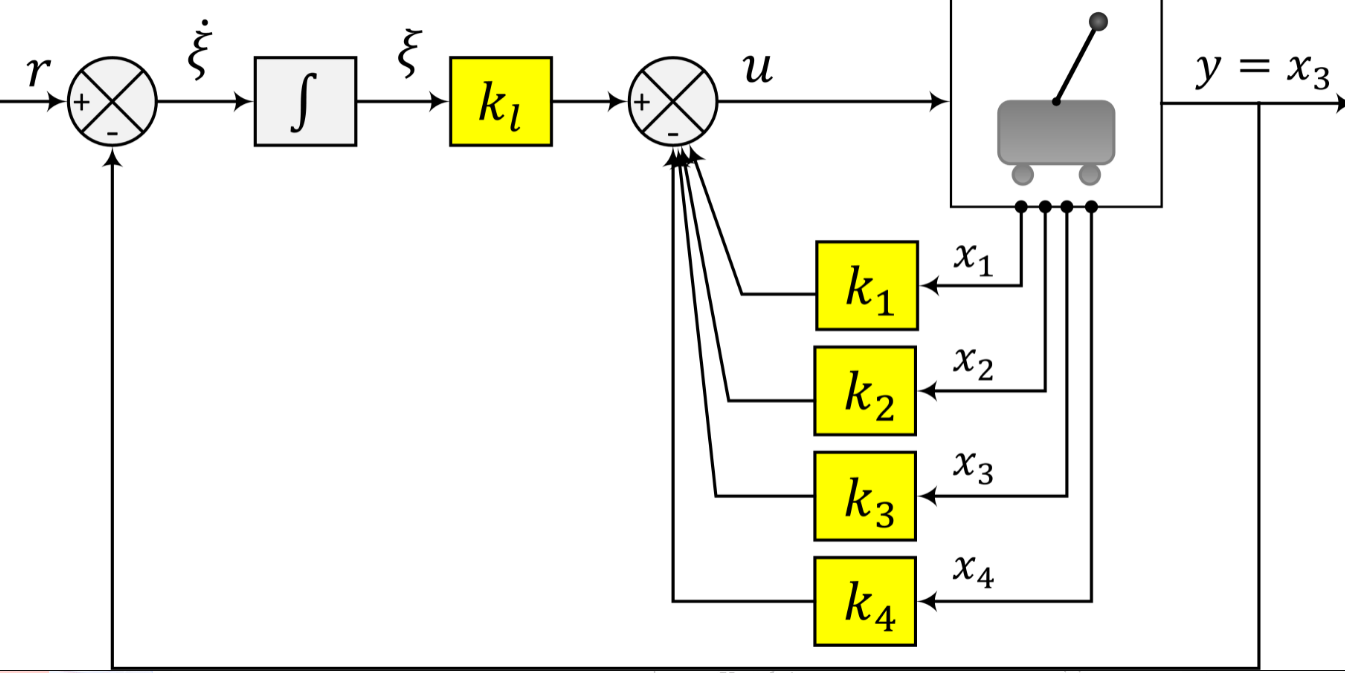
\includegraphics[width=0.55\linewidth]{倒立摆闭环框图}
				\caption{倒立摆闭环框图}
				\label{fig:倒立摆闭环框图}
			\end{figure}\par
			根据上图的系统框架，可以推导闭环系统的方程描述：
			\begin{gather}
				\begin{cases}
					\dot{x}=Ax+Bu\\
					y=Cx\\
					u=-Kx+k_I\xi\\
					\dot{\xi}=r-Cx\\
				\end{cases}
			\end{gather}\par
			将上式合并处理，得到系统动态特性的方程描述：
			\begin{gather}
				\begin{bmatrix}
					\dot{x}(t)\\
					\dot{\xi}(t)\\
				\end{bmatrix}
				=
				\begin{bmatrix}
					A&0\\
					-C&0
				\end{bmatrix}
				\begin{bmatrix}
					x(t)\\
					\xi(t)\\
				\end{bmatrix}
				+
				\begin{bmatrix}
					B\\
					0\\
				\end{bmatrix}
				u(t)+
				\begin{bmatrix}
					0\\
					1
				\end{bmatrix}
				r(t)
			\end{gather}\par
			计算得到重构矩阵的秩$r=5$（代码见附录），由于闭环系统为$5$阶，因此，上述系统的状态是完全可控的，进而可以对系统进行任意极点配置，行系统极点配置设计，以得到控制律$u$。实际上就是根据状态方程以及目标极点位置，来计算控制律$u$中状态反馈增益$K$及前向积分增益的值。\par
			我们知道系统闭环极点的位置决定了其时域响应特性，由于闭环系统的阶次为$5$，需要为其配置$5$个极点，为保证系统的响应性能，配置其中$2$个极点为主导极点（方程$s^2+2\times0.7s+1=0$ 的共轭复根，即阻尼为$0.7$的理想二阶环节极点），并使其余$3$个极点远离主导极点$(-10,-15,-20)$。采用控制系统工具箱的place 函数，计算满足主导极点位置的状态反馈增益及前向积分增益。\par
			计算得到状态反馈增益$K=[k_1 \quad k_2 \quad k_3 \quad k_4]$及前向积分增益$k_l$ 分别为：$-982.029$、$255.995$、$-494.898$、$-419.19$、$-306.1224489795918$。\par
			将所设计的控制律$u=-Kx+k_l\xi$带入式，得到闭环系统的状态方程为：
			\begin{gather}
				\begin{bmatrix}
					\dot{x}\\
					\dot{\xi}\\
				\end{bmatrix}
				=
				\begin{bmatrix}
					A-BK&Bk_l\\
					-C&0
				\end{bmatrix}
				\begin{bmatrix}
					x\\
					\xi\\
				\end{bmatrix}
				+
				\begin{bmatrix}
					0\\
					1
				\end{bmatrix}
				r
			\end{gather}\par
			系统的输出为小车的平衡位置$x_3$，即：
			\begin{gather}
				y=
				\begin{bmatrix}
					0&0&1&0&0\\
				\end{bmatrix}
				\begin{bmatrix}
					x\\
					\xi
				\end{bmatrix}
			\end{gather}\par
		\subsection{系统仿真}
			首先在Mworks的Sysplorer仿真平台上搭建原系统在没有进行状态反馈时的数学模型：
			\begin{figure}[H]
				\centering
				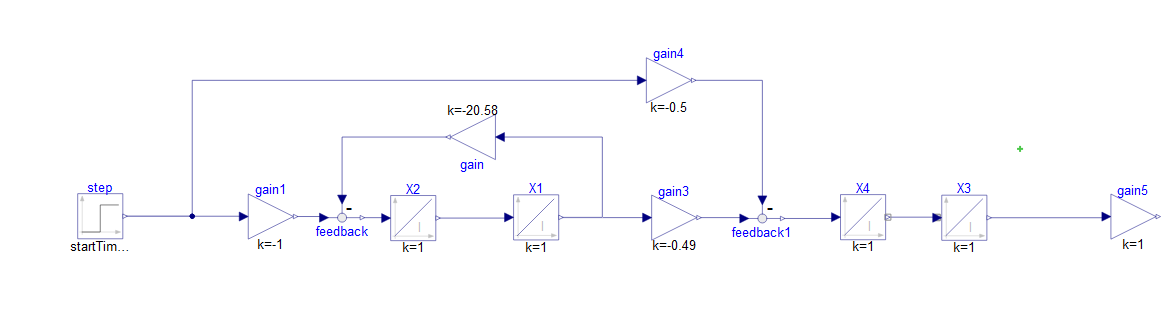
\includegraphics[width=0.8\linewidth]{未状态反馈时数学模型}
				\caption{未状态反馈时数学模型}
				\label{fig:未状态反馈时数学模型}
			\end{figure}\par
			经过调试，未状态反馈时系统仿真结果如下图所示：
			\begin{figure}[H]
				\centering
				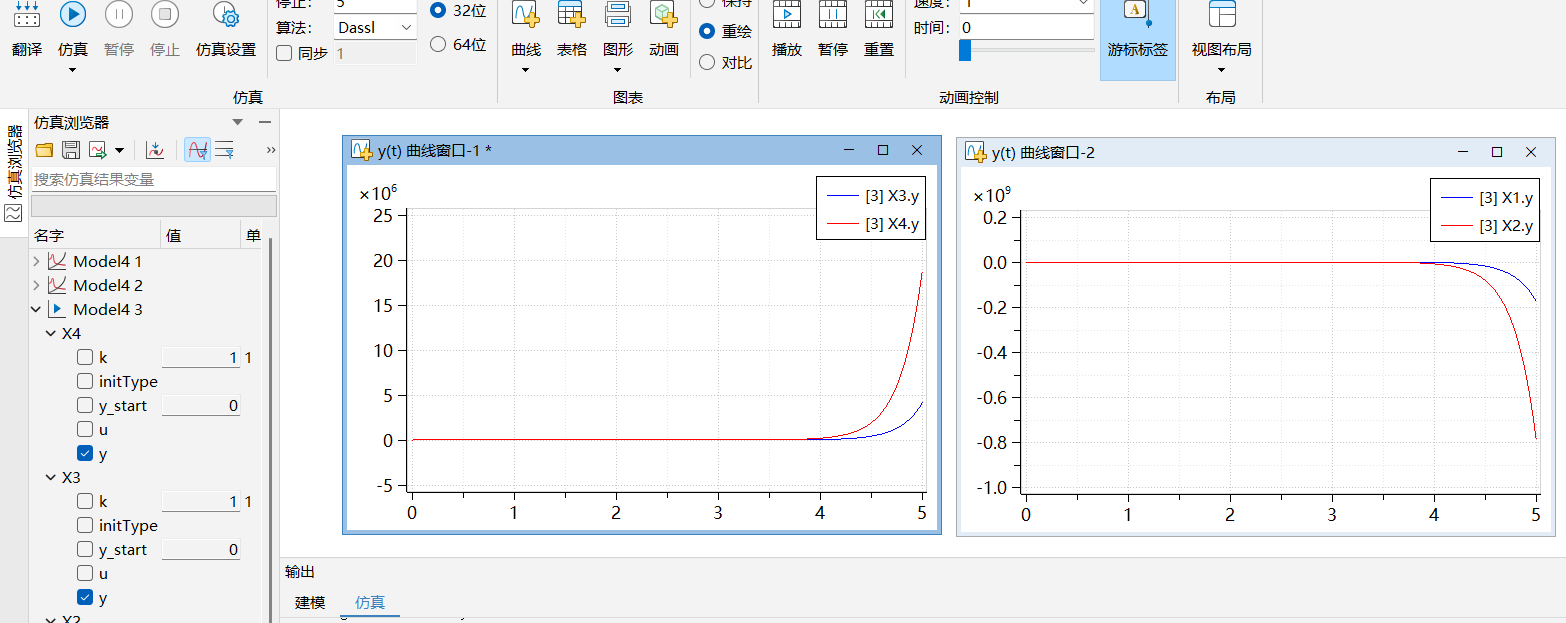
\includegraphics[width=0.8\linewidth]{未状态反馈时系统仿真结果}
				\caption{未状态反馈时系统仿真结果}
				\label{fig:未状态反馈时系统仿真结果}
			\end{figure}\par
			由响应曲线可见，在未进行状态反馈时，系统在阶跃信号的输入作用下，小车的位移和摆杆的角度全部都是发散的，会一直运动下去，即系统是不稳定的，需要进行状态反馈。\par
			由于原系统是不稳定的，要使系统稳定,需要加入状态反馈，使系统的极点全部位于左半平面，控制系统的各种特性及其品质指标在很大程度上是由其闭环系统的零点和极点的位置决定。极点配置问题就是通过对状态反馈矩阵的选择，使其闭环系统的极点配置在所希望的位置上，从而达到期望的性能指标的要求。由于系统完全能控，可以通过状态反馈来任意配置极点。状态反馈的结构图如图\ref{fig:未状态反馈时数学模型}所示：
			\begin{figure}[H]
				\centering
				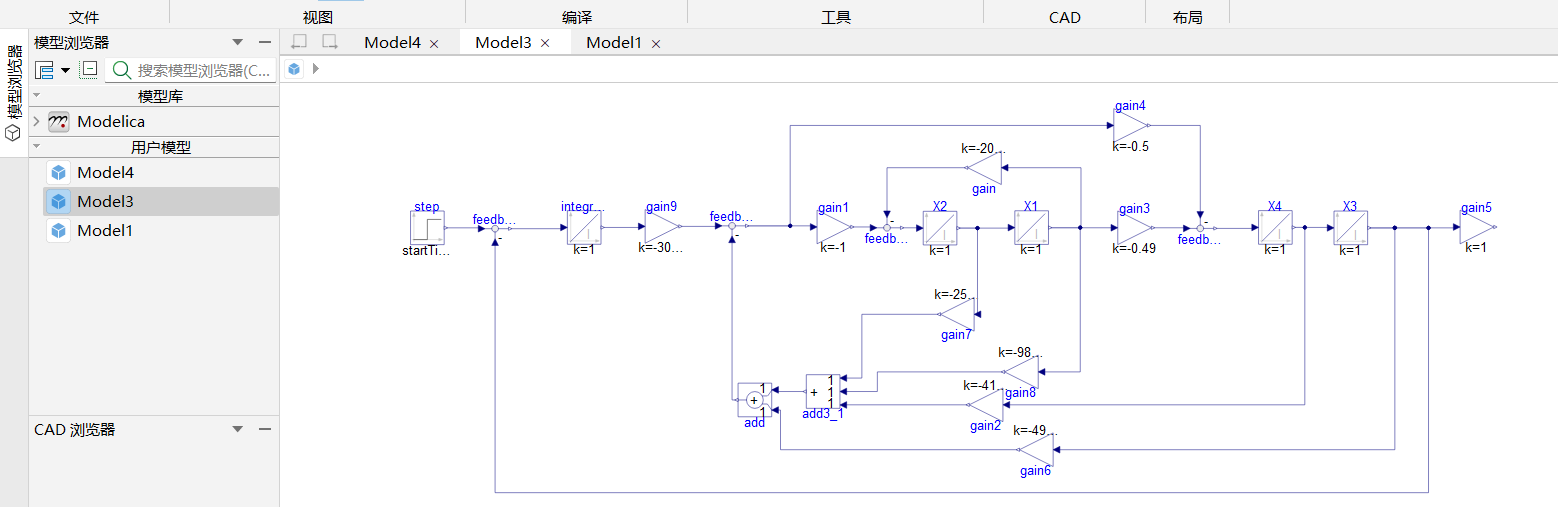
\includegraphics[width=0.8\linewidth]{状态反馈时数学模型}
				\caption{状态反馈时数学模型}
				\label{fig:状态反馈时数学模型}
			\end{figure}\par
			由此得到的系统状态反馈数学模型响应曲线如下图所示：
			\begin{figure}[H]
				\centering
				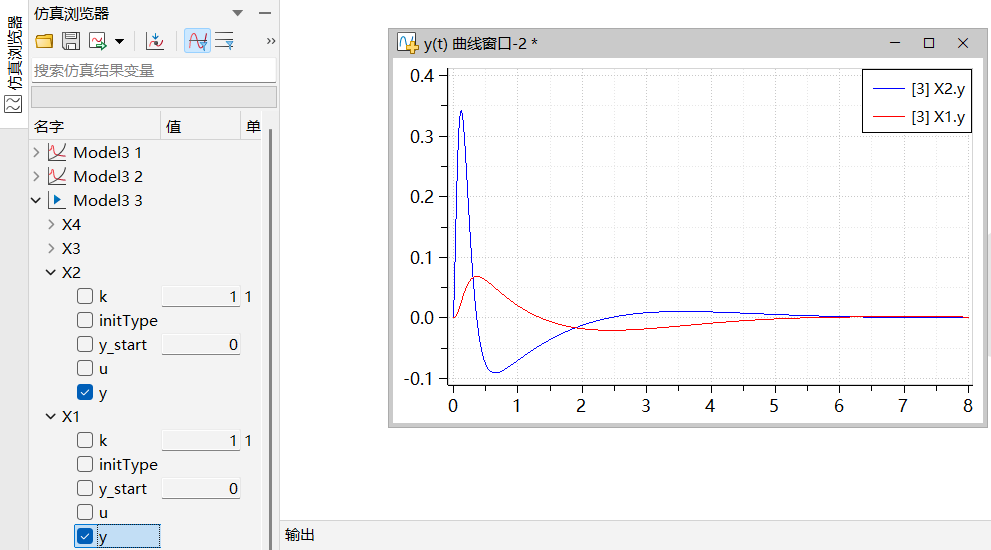
\includegraphics[width=0.8\linewidth]{角度和角速度响应曲线}
				\caption{角度和角速度响应曲线}
				\label{fig:角度和角速度响应曲线}
			\end{figure}\newpage
			状态反馈数学模型位移和速度响应曲线：
			\begin{figure}[H]
				\centering
				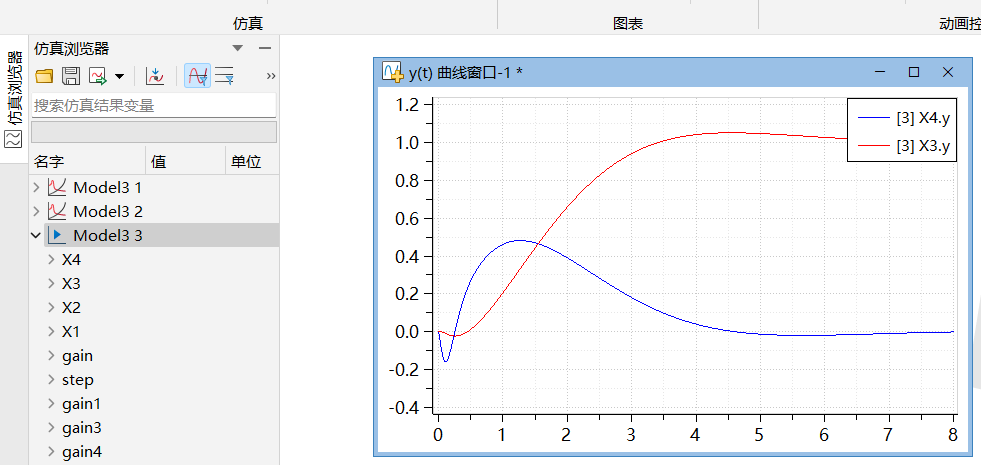
\includegraphics[width=0.8\linewidth]{位移和速度响应曲线}
				\caption{位移和速度响应曲线}
				\label{fig:位移和速度响应曲线}
			\end{figure}\par
			由系统的响应曲线可知，在原来的阶跃响应输入下，经过三秒左右的时间之后，摆杆的角度和角速度均为零，摆杆稳定在垂直状态，这说明加入状态反馈后可以使原系统达到稳定状态。\par
			系统状态反馈之后的物理模型搭建：
			\begin{figure}[H]
				\centering
				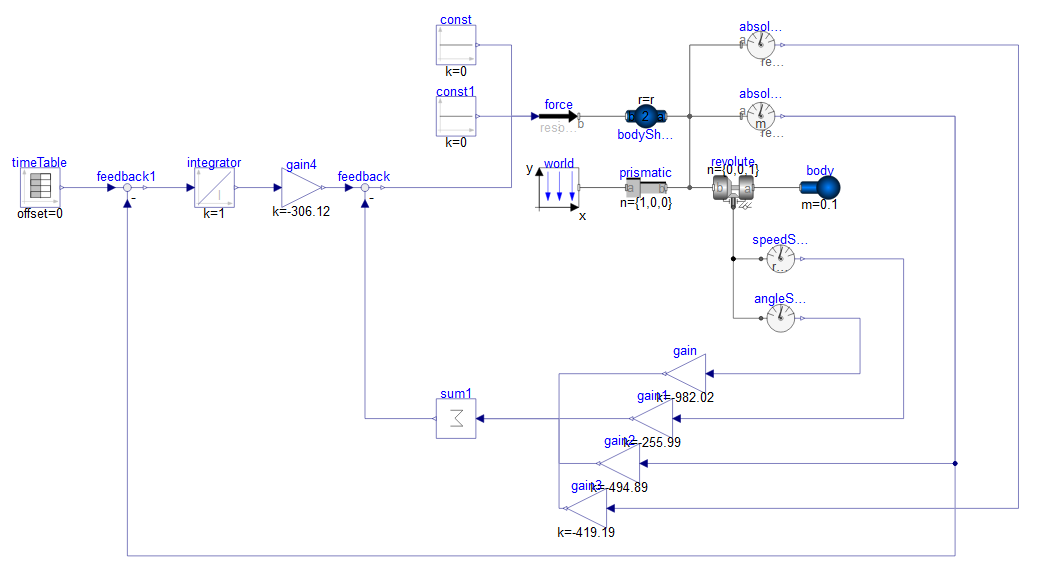
\includegraphics[width=0.8\linewidth]{状态反馈时物理模型}
				\caption{状态反馈时物理模型}
				\label{fig:状态反馈时物理模型}
			\end{figure}\newpage
			经过仿真之后的系统物理模型响应曲线如下：
			\begin{figure}[H]
				\centering
				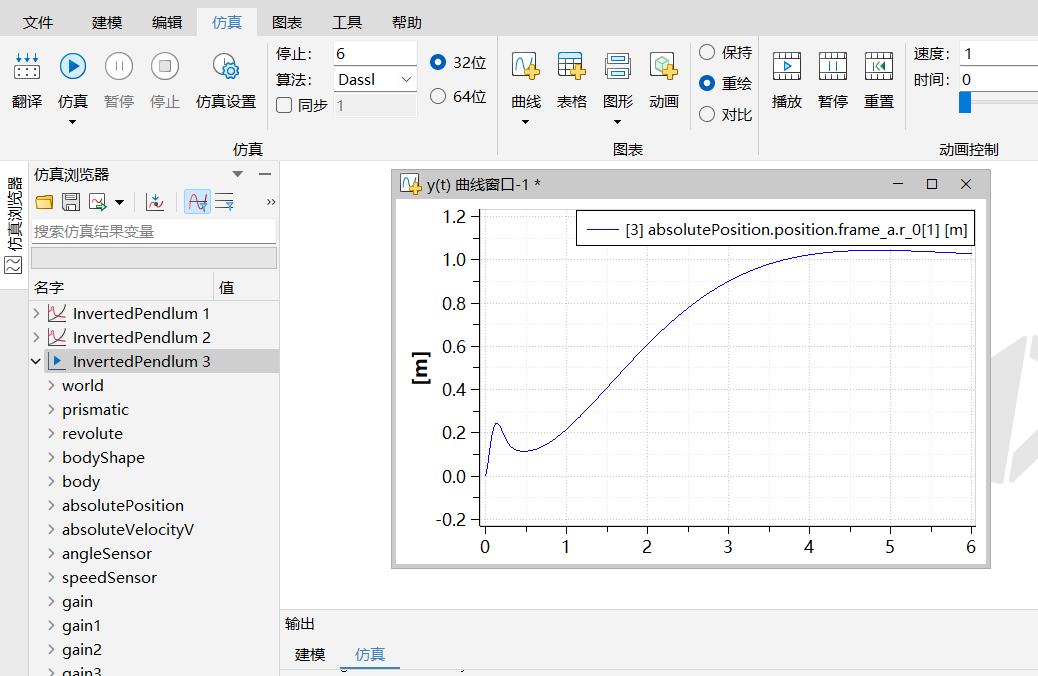
\includegraphics[width=0.8\linewidth]{位移响应曲线}
				\caption{位移响应曲线}
				\label{fig:位移响应曲线}
			\end{figure}\par
			系统物理模型速度响应曲线:
			\begin{figure}[H]
				\centering
				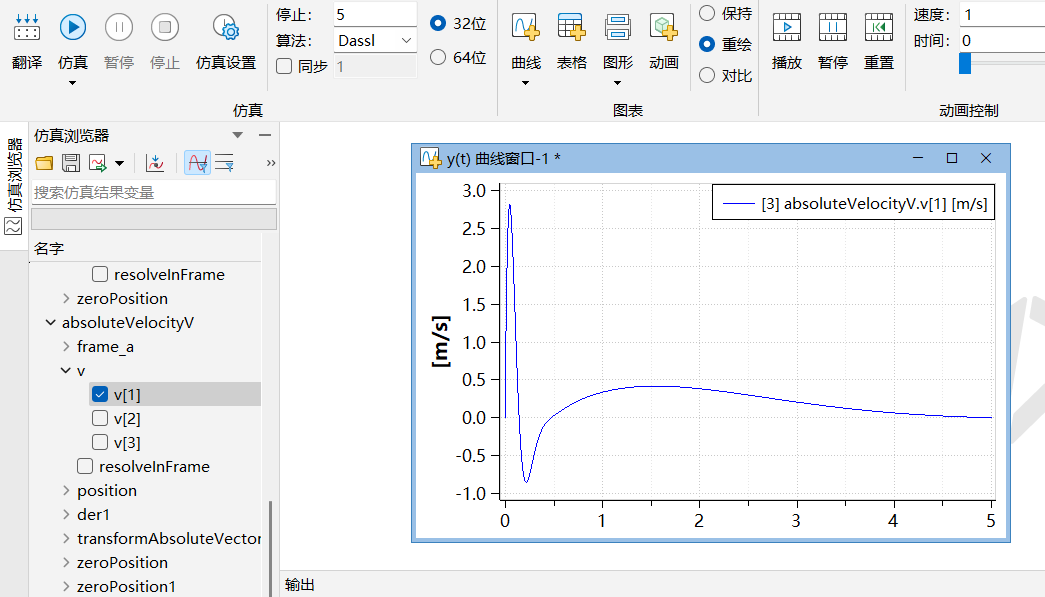
\includegraphics[width=0.8\linewidth]{速度响应曲线}
				\caption{速度响应曲线}
				\label{fig:速度响应曲线}
			\end{figure}\par
			\newpage
			物理模型角度和角速度响应曲线:
			\begin{figure}[H]
				\centering
				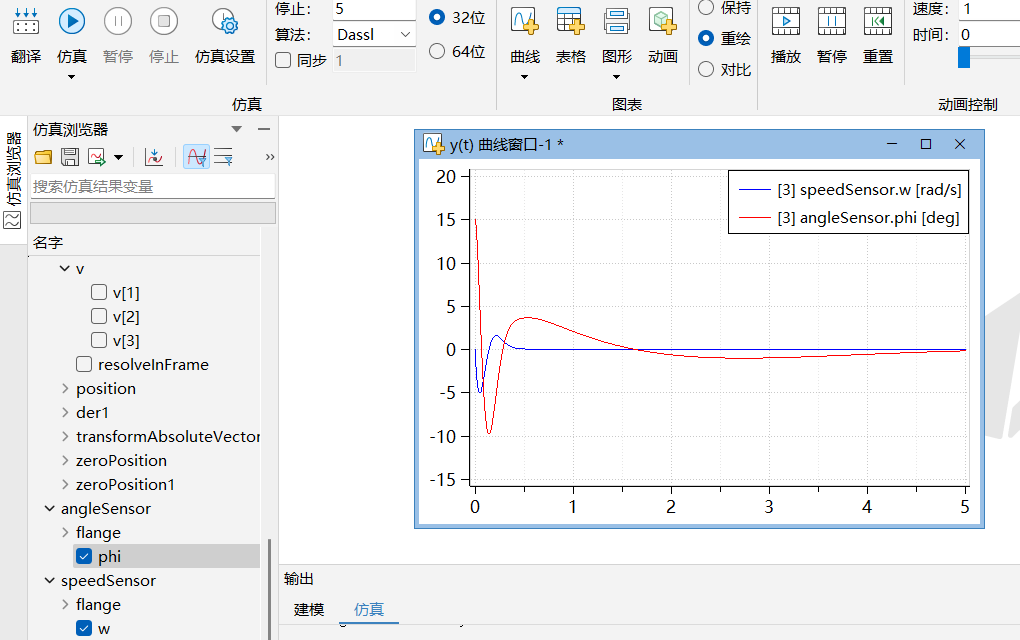
\includegraphics[width=0.8\linewidth]{角速度和角度响应曲线}
				\caption{角速度和角度响应曲线}
				\label{fig:角速度和角度响应曲线}
			\end{figure}\par
			由以上结果可见，物理模型的仿真结果与数学模型一致，在经过状态反馈之后，倒立摆底座的位移、速度以及摆杆的角度均在$3$s之后逐渐趋于稳定。可见，在控制律作用下，摆杆摆角在$6$s 左右调整为$0^\circ$，小车同样在$6$s 左右在$x=1$的位置平衡。通过系统闭环阶跃响应，系统稳态误差为$0$，超调较小且响应快，因此，控制效果较好
			
			
			
			
	\section{心得体会}
		倒立摆系统仿真是一个复杂而具有挑战性的工程实践，它不仅让我们团队更深入地理解了物理原理，也让我们切身感受到现代控制理论在实际应用中的意义。在整个从理论学习到实践的过程中，我们积累了一些经验和心得：
		
		\paragraph{理论与实践的结合}\qquad 在倒立摆系统的建模过程中，首先需要通过物理分析建立出系统的状态空间模型，这是现代控制理论的基础。状态空间模型的建立帮助我们将物理过程转化为数学形式，从而能够进一步精细量化对系统的控制。通过状态空间模型的描述，我们能够分析出系统的能控性和能观性，深入了解系统的动态变化。控制理论的有效性在于能够通过状态反馈控制和极点配置等方法，将理论上的模型应用于实际控制中。在仿真过程中，我们逐步实现了从建模到应用的全过程，强化了理论与实践的结合。
		\paragraph{系统稳定性与控制的精细调节}\qquad
		倒立摆系统的控制需要对稳定性进行精细调节，这正是现代控制理论中的一大优势。通过求解状态方程，我们能够明确系统的动态响应并掌握其稳定性。在控制过程中，使用极点配置和状态反馈控制方法，我们能够根据系统的特性设计合适的控制器，以实现系统的稳定性。这不仅要求精确的数学推导，也要求我们灵活运用这些理论在复杂的系统中进行调试和优化。例如，在系统的精细调节中，如何调整反馈增益以平衡快速响应和稳定性，就是对理论应用的一种挑战。
		\paragraph{仿真工具的使用与提升}\qquad
		在仿真过程中，Mworks仿真软件的使用使我们能够快速建立状态空间模型，并进行数值求解。通过计算状态转移矩阵，我们能够获得系统在不同时间下的状态演变，进一步验证控制算法的有效性。此外，仿真工具不仅帮助我们实现了控制策略的测试，也加深了我们对能控性和能观性的理解。例如，验证系统是否能通过适当的输入控制到任意状态，或是能否通过观测输出推测系统内部状态，这些都是控制设计中的关键环节。
		\paragraph{问题解决与创新能力的培养}\qquad
		在仿真过程中，面对如模型不精确或控制算法不稳定等问题，我们运用了状态观测器来弥补系统测量不足的问题。通过设计状态观测器，我们能够准确估计系统的内部状态，从而提高控制精度。在这一过程中，控制方法的正确运用能够有效应对实际问题中的不确定性。这不仅是对控制理论的深度应用，也是在复杂环境下提升系统性能的一个有效手段。
		\paragraph{团队合作与沟通的意义}\qquad
		在团队协作中，控制系统的设计往往涉及多个方面的知识整合。团队成员通过共同讨论状态空间模型的建立、状态反馈的设计以及极点配置等控制策略的应用，每个人的对问题的理解和想法得到了充分沟通。清晰的分工和有效的沟通使得理论知识能够更快速地转化为具体的实施方案。在设计和调试过程中，能够有效地交换意见，提出不同的理论观点，并协作解决实际问题，是推动项目顺利进行的重要因素。
		\paragraph{工程实践与全面发展的启示}\qquad
		在倒立摆仿真实践过程中，我们深刻认识到跨学科的知识整合对于工程实践的必要性。除了控制理论的学习，我们还需要掌握如何从物理模型建立状态方程、如何使用编程语言实现控制算法、如何运用数值分析方法解决实际问题等技能。
		
		
	
	\newpage
	\appendix
	\section*{附录A \quad 代码}
		\begin{lstlisting}[language={}]
using TyControlSystems
using TyMath
using TyPlot
# 倒立摆系统参数
M = 2     # 小车质量2Kg
m = 0.1   # 摆球质量0.1Kg
l = 0.5   # 摆杆长度0.5m
g = 9.8   # 重力加速度9.8m/s^2
# 倒立摆系统状态空间矩阵定义
A = [0 1 0 0
(M+m)*g/(M*l) 0 0 0
0 0 0 1
-m*g/M 0 0 0]
B = [0 -1 / (M * l) 0 1 / M]'
C = [0 0 1 0]
D = 0
# 倒立摆系统模型
G = ss(A, B, C, D)
#绘制系统零极点图
pzmap(G)
#能控能观性判别
Co = ctrb(G)
Ob = obsv(G)
r1=rank(Co)
r2=rank(Ob)
#状态模型转化为zpk模型
Gzpk = zpk(G)
# 0型系统重构
Ahat = [A zeros(size(A, 1), 1); -C 0]
Bhat = [B; 0]
#判定重构系统能控性
r = rank([Ahat Bhat])
# 计算理想主导极点位置并分配系统所有极点位置
idealPoles = roots([1, 2 * 0.7 * 1, 1])
AllPoles = [idealPoles[1], idealPoles[2], -10, -15, -20]
# 极点配置，计算状态增益K
Khat = place(Ahat, Bhat, AllPoles)
# 状态增益值分解
K = reshape(real(Khat[1:4]), 1, 4)
k1 = -real(Khat[end])
# 闭环系统状态方程
AA = [A-B*K B*k1; -C 0]
BB = [0 0 0 0 1]'
CC = [C 0]
DD = 0
Gclose = ss(AA, BB, CC, DD)
# 计算并绘制阶跃响应
#step(Gclose, 10, linewidth = 2) 
#y, t, x = step(Gclose, 10)

		\end{lstlisting}
	
\end{document}









